\section{Introduction}
The introduction of hardware HEVC encoders to consumer-grade GPUs has opened the door to mass 360-degree and 4K video livestreaming, but does not immediately offer a solution to adaptive video streaming. Recently, a significant body of work on tile-based adaptive streaming for 360-degree and 4K video has appeared, in which the quality requested for each section of a video corresponds to how interesting it is, allowing clients to view the most important parts of a video, or, e.g., those which a user is moving their head towards, in high-quality without stalling. This is straightforward for pre-rendered video, but is more complicated in a livestreaming scenario because each quality requires another encode, necessarily introducing some delay in the availability of a new segment. Furthermore, tiling, which must occur within the HEVC encoder prior to generation of the bitstream, is not supported by existing hardware encoders. One can try to get around this by feeding each tile to the encoder as a separate video and stitching them together afterwards, but even top-of-the-line consumer-grade GPUs only support two contiguous encoding processing, forcing the user to either encode the whole frame at two different qualities, or divide each frame into two tiles but only offer a single quality for either tile. In the former case, tiling does not occur; in the latter, the tile sizes are so large as to render the point moot, and the video stream is not adaptive because only one quality is available for either half.

To combat these challenges, we introduce WORKINGTITLE, a GPU-based HEVC encoding pipeline to tile, encode, and stitch video at multiple qualities in real-time on a frame-by-frame basis. WORKINGTITLE uses HEVC slices in conjunction with tiles to encode each region of a video independently, so that a player can pick and choose which quality they want for each region. To do so, the source video stream is divided into vertical strips, which are stacked on top of one another. This restructured video image is fed to the encoder with slice boundaries specified to at least be the edges of these strips, so that each slice is some fraction of the horizontal width and, possibly, vertical height. This process occurs twice for each frame, resulting in high-quality and low-quality outputs. When the video is reconstructed during playback, each slice is an independently-decodable region of video, so we are free to pick and choose either quality for each region of the video shown to the user.

\begin{figure*}[t]
	\centering
	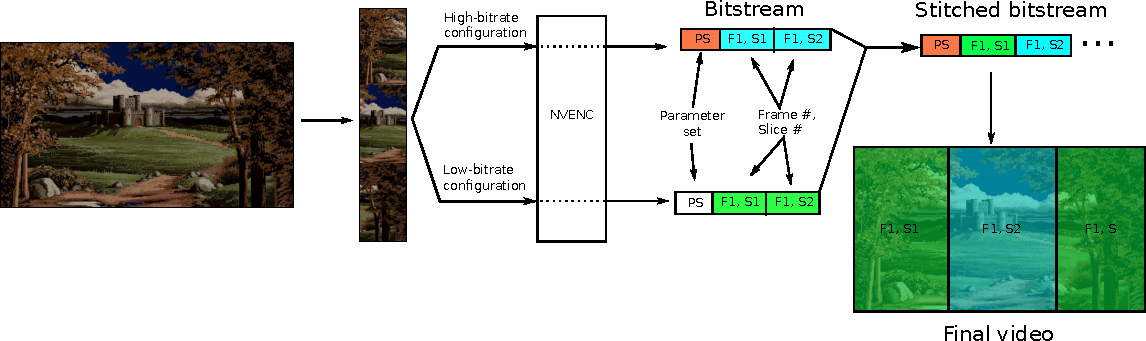
\includegraphics[width=\textwidth]{figures/pipeline.pdf}
	\caption{An illustration of the pipeline}
\end{figure*}

The rest of this paper is organized as follows: ...

\section{HEVC and NVENC}

The most computation-heavy components of the HEVC encoding process, such as motion estimation, are not easily parallelized. Parallel HEVC video encoding instead relies on dividing each frame of the video into independent regions, encoding them separately, and joining their edges during playback. Two versions of this concept, slices and tiles, exist within the HEVC standard. Functionally, they are identical; however, slices are limited to chunking the video into wide strips, while tiles can divide a video into rectangular CTU-based areas of any size. While tiles are supported by most decoders, very few encoders allow for it, all of which are software encoders far too slow to operate in real-time. 

HEVC encoders convert raw video into an HEVC bitstream consisting of multiple sequential NAL units via a complex implicit syntax. Each NAL unit contains some header information followed by raw image data. For videos without slicing or tiling, most NAL units correspond to a single full frame of video; however, because slices and tiles are independently-decodable, each tile or slice within a video frame is a self-contained NAL unit. Interestingly, we can then treat any rectangular arrangement of HEVC bitstreams as tiles within a single video by alternating their NAL units and manipulating specific values in the NAL headers. This process, in which multiple bitstreams are joined to form one bitstream which displays all constituent bitstreams in different regions of the final video, is known as \textit{stitching}. (Maybe include some references to works which do stitching or something)

NVENC is a hardware video encoder present on newer Nvidia GPUs, and is the state-of-the-art hardware HEVC encoder. Note that HEVC is not easily data-parallelizable; as a result, NVENC is an ASIC separate from the CUDA cores. Interaction with NVENC occurs via the NVENCODE API, and offers the user a handful of parameters for the encoder, such as target bitrate, slice boundaries, and GOP specifications. It is possible to swap out encoder configurations between frames, allowing one to encode multiple videos simultaneously, but even top-of-the-line consumer GPUs only support a maximum of two contiguous configurations. Note that these configurations are not simply encoding parameters, but also contain, e.g., the previous frame data necessary to encode the next P- or B-frame. This is a limitation enforced by the driver, and supercomputing GPUs, such as the Nvidia Titan V, do not have such limits. Unfortunately, such GPUs are prohibitively expensive and overpowered for most use cases, so we do not consider them here.

\section{WORKINGTITLE Implementation}
- Briefly mention Kvazaar and FFmpeg \\
- Restructuring the input and passing it to NVENC \\
- Stitching the bitstream

To work within the confines imposed by NVENC, namely the lack of tile support and limitation to two simultaneous encoding sessions, we divide the real-time encoding and playback pipeline into an encoding component, in which a raw video frame is manipulated and converted into a bitstream, and a stitching component, in which these bitstreams are combined to be displayed to the user.

\subsection{Encoding}
NVENC supports multiple slice modes, one of which, \texttt{sliceMode=3}, cuts the video into $n$ equal slices as specified via the \texttt{sliceModeData=}$n$ parameter. Vertical cuts, which are important for 360-degree video, cannot be made via slices, but the image boundaries are natural slice boundaries as well. We therefore manipulate the input images by vertically slicing them into thirds and stacking these slices on top of each other, then setting \texttt{sliceModeData=}$3$, so that the slice boundaries align with the top and bottom boundaries of the original image. The output bitstream from the encoder will then contain three NAL units per frame, one for each slice. During the stitching process, specific changes will be made to the NAL headers to instead treat these slices as tiles and place them side-by-side in the final video bistream.

To stream different regions at different quality levels, we encode the restructured input frames at two different target bitrates.

\subsection{Stitching}

\section{Installing and Using WORKINGTITLE}
Configuring and using the software. Some implementation stuff could go here for our actual demo (e.g. using it while streaming with a real camera).

\section{Evaluation}
- Tradeoff between tile size and coding/network transmission efficiency \\
- Maybe encoding presets? We could find the best presets to use for the low/high settings based on output size, perceived quality (PSNR), encoding speed, etc.

\section{Conclusion}